\documentclass[reqno,14pt]{amsart}
\usepackage{amsmath,amssymb,amsthm, mathtools, verbatim, graphicx, url, pinlabel, float, biblatex, subfig, epigraph}
\usepackage[justification=centering]{caption}
\usepackage[usenames, dvipsnames]{color}

\usepackage[letterpaper,hmargin=1in,vmargin=1in]{geometry}
\usepackage[framed,numbered,autolinebreaks,useliterate]{mcode}

\newcommand{\mar}[1]{{\marginpar{\sffamily{\tiny #1}}}}

\usepackage{graphicx}
\usepackage{enumitem,pinlabel}
\setlist{  
  listparindent=\parindent,
  parsep=0pt,
}
\usepackage{mathrsfs,graphicx,url}
\usepackage[usenames,dvipsnames]{xcolor}
\usepackage[colorlinks=true,linkcolor=Black,citecolor=Black, urlcolor=Black]{hyperref}

\theoremstyle{plain}
\newtheorem{theorem}{Theorem}
\newtheorem*{theorem*}{Theorem}
\newtheorem*{lemma*}{Lemma}
\newtheorem*{proposition*}{Proposition}
\newtheorem*{corollary*}{Corollary}
\newtheorem{lemma}{Lemma}[section]
\newtheorem{proposition}[lemma]{Proposition}
\newtheorem{corollary}[lemma]{Corollary}
\newtheorem{fact}{Fact}[subsection]

\theoremstyle{definition}
\newtheorem{definition}{Definition}[subsection]
\newtheorem{example}{Example}[subsection]
\newtheorem{method}{Method}[subsection]
\theoremstyle{remark}
\newtheorem{claim}{Claim}[subsection]
\newtheorem{question}{Question}[subsection]
\newtheorem{note}{Note}[subsection]



\title{Pricing European Options with Neural Networks}
\author{CJ Destefani, Financial Mathematics MS}
\date{December 5, 2022}

\begin{document}

\maketitle
\section{Abstract}
This project uses both Matlab's built in Neural network toolbox and a custom-made neural network with a single hidden layer for the purpose of pricing European options. The ground truth values used for training and testing these networks were obtained from the Black-Scholes-Merton equation for European options. This equations is 
\begin{equation}
    BSC(S,T,K,r,\sigma,q) = S e^{-qT} N(d_1) - K e^{-r T}N(d_2)
\end{equation}
where 
\begin{equation}
    d_1 = \frac{\ln(\frac{S}{K}) + (r -q -\frac{1}{2}\sigma^2) T}{\sigma \sqrt{T}}, \quad d_2 = d_1 - \sigma \sqrt{T}
\end{equation}
and
\begin{equation}
    N(y) = \frac{1}{\sqrt{2 \pi}} \int_{-\infty}^y e^{\frac{-1}{2} u^2} du
\end{equation}
which is conveniently implemented in Matlab with the function `blsprice'. However, instead of using 6 input variables, we can combine the stock price ($S$) and the strike price ($K$) into one quantity: Moneyness. It is defined as $\frac{S}{K}$. It slightly modifies our BSC equation as follows:
\begin{equation}
    BSC(\frac{S}{K},T,1,r,\sigma,q) = \frac{BSC(S,T,K,r,\sigma,q)}{K}.
\end{equation}

We decided to calculate 20,000 data points with various values of moneyness ($\frac{S}{K}$), maturity time ($T$), interest rate ($r$), volatility rate ($\sigma$), and dividend rate ($q$). These parameters were chosen in a pseudo-random fashion using a five dimensional Sobol set that received a random linear scramble combined with a random digital shift. This set of inputs was then used to calculate the `exact' price with blsprice, and then these same input values were used as input to our neural networks. The specific parameter ranges used are as follows:
\begin{center}
\begin{tabular}{||c c c||} 
 \hline
 Parameter & Lower bound & Upper bound \\ [0.5ex] 
 \hline\hline
 Moneyness & 0.5 & 5 \\ 
 \hline
 Maturity time (years) & .1 & 2 \\
 \hline
 Interest rate (\%) & 1 & 10 \\
 \hline
 Volatility rate (\%) & 5 & 50\\
 \hline
 Dividend rate (\%) & 0 & 3\\
 \hline
\end{tabular}
\end{center}


The loss function for both networks was the MSE (mean squared error) given as:
\begin{equation}
    L(y,\hat{y}) = \frac{1}{N} \sum_{i=1}^N (y_i - \hat{y_i})^2.
\end{equation}
Then, of course, the goal is the minimize this $L$. We, as users, can tweak the network's structure and hyperparameters to do this, but the computer will do the majority of the work by optimizing the parameters (weights and biases) of the network once you push `run'. \\


\section{Matlab's built in Neural Network Functions}
Because the example given on Matlab's website (at https://www.mathworks.com/help/fininst/deep-learning-to-approximate-barrier-option-pricing.html) is so complete, it was relatively easy to modify the code to predict the prices of even simpler options--European calls. But having the code allowed one to play with all of the structural elements, hyperparameters, and activation functions that would otherwise be very difficult to discover or make from scratch.\\
The first observations were that the number of neurons in the hidden layer did improve the final loss (more neurons caused a lower loss and thus more accurate performance), but not by as much as we initially expected. 100 neurons (i.e. a network width of 100) gave the lowest losses, but shrinking it down to 50 neurons gave performance that was within a few percentage points.\\
Next we noticed that the activation functions had a very large effect on the network's performance. Initially, we assumed that the sigmoid would be as good a choice as any for both activation functions since it is a $C^\infty$ function and has nice derivatives, but this turned out to be quite limiting. Since the sigmoid is given by:
\begin{equation}
    f(x) = \frac{1}{1+e^{-x}},
\end{equation}
its range is contained in the unit interval. Thus, if this function is used at the final layer, all of the option prices obtained from the network will, necessarily, be between zero and one! Sorting out this limitation, ReLu (Rectified Linear Unit) turned out to be a much better activation function for both layers. With this set up, it was common to achieve a final loss of less than $10^{-3}$.\\
Then, we examined the relationship between the number of hidden layers. This, like the number of neurons, did not affect the performance as much as we initially expected, but on the whole did make a large contribution to decreasing the network's overall loss. The optimal number of layers was found to be about 6 with the average loss increasing on both sides of that.\\
With all of these optimizations, the average loss is approximately $3*10^{-4}$ on the final data set. At a single layer, the network runs in as little as 18 seconds, and with 6 layers, it runs in 33-69 seconds depending on the width and hyperparameters.\\

\section{Custom Neural Network--Derivation}
Instead of simply using the tool kits for machine learning in Matlab, the process of deriving, designing, and programming a neural network by hand was a valuable learning experience as it required a working knowledge of all the necessary components.\\

So why should we use a neural network to price options at all? The universal approximation theorem tells us that the network can approximate the Black Scholes equations, and thus provides an alternative pricing approach to Monte Carlo simulation and other pricing techniques. As discussed in lectures, the \textit{Universal Approximation Theorem} applies to any neural network that has a single hidden layer provided its depth is sufficiently large. In particular, it states that a neural network with a single hidden layer with a large number of neurons and activation functions that are continuous, bounded, and non-constant can approximate any function arbitrarily closely.\\

\subsection{How Neural Networks Work}
A neural network operates, most basically, by tuning many different parameters that allow a large composite function to approximate an arbitrary function. Such parameters include weights and biases that are combined in a weighted sum at each neuron. After each neuron in a layer has a value, they are `activated' meaning they are put through a nonlinear activation function. This step gives the network the ability to approximate nonlinear functions in an otherwise linear set up.\\
The structure of our neural network is not complicated. The first layer corresponds to the input layer; here each input variable gets its own neuron. The final layer corresponds to the output layer and is a single neuron since we only have one output: the option price (divided by the strike price, in this case). The hidden layer (assume there is only one for our construction) has $J$ neurons in it. Each of these $J$ neurons connects to all 5 input neurons, and each such connection has an associated weight. The weight connecting the $i^{th}$ input to the $j^{th}$ neuron is $w^0_{i,j}$. Each hidden layer neuron also has a bias associated with it, called $b^0_j$. The weighted average of these input layer values, weights, and biases will provide the values at each neuron of the hidden layer. This is written mathematically as follows: 
\begin{equation}
    \hat{y}^0_j = \Psi_0( b^0_j + \sum^5_{i=1} w^0_{i,j} x_i )
\end{equation}
where $\hat{y}^0_j$ is the number in the $j^{th}$ neuron of the hidden layer and $\Psi_0$ is the initial activation function. We include hats on the $y$'s because these are approximations from the network (and not the exact values which are denoted without hats and are given by the Black Scholes equations). This means that to go from the input layer to the hidden layer, there are $5J$ weights and $J$ biases for a total of $6J$ parameters so far. Next, we need to connect the hidden layer to the output layer. Since the output layer is, in our case, just one neuron, we connect all $J$ hidden neurons to it. These connections are weights in the same manner and are called $w^1_j$. Additionally, the final neuron has one final bias associated with it called $b^1$. These are combined as follows: 
\begin{equation}
    \hat{y} = \Psi_1( b^1 + \sum^J_{j=1} w^1_j \hat{y}^0_j )
\end{equation}
where $\hat{y}$ is the final price prediction of the option price and $\Psi_1$ is the final activation function. Multiplying this number by $K$ (the strike price) will give you the untransformed option price. This final layer adds an additional $J+1$ parameters for the model to optimize for a total of $7J+1$ parameters.\\

We will discuss the optimization process in the next subsection, however, as this is quite involved and depends on the activation functions used. To continue, lets discuss instead how to make this computationally feasible. If I told a computer to solve the two above equations, it could, but not optimally because it would handle each option's inputs and prices in a vacuum; matrices are much more efficient ways of multiplying and adding many things together. As this would suggest, let's vectorize everything and try to rewrite the above equations more succinctly. If we have a dataset size (or batch size) of $M$, this allows us to define a matrix of input values $\overrightarrow{x}_{5 \times M}$. The subscripts here indicate the size of the resulting matrix. Similarly, the hidden layer's values $\hat{y}^0_j$ depend on both $J$ and $M$, so all of those values can be put into $\overrightarrow{\hat{y}^0} _{J \times M}$. The output layer's values only depend on $M$, so it will become $\overrightarrow{\hat{y}}_{1 \times M}$. Meanwhile, the weights and biases will be the same for each option and thus should not depend on $M$; the weights connecting the input and hidden layers depends on the size of each, so this becomes a matrix $W^0_{J \times 5}$. The biases for that layer depend only on the depth $J$, so this becomes a vector $\overrightarrow{b^0}_{J \times 1}$. As will be seen soon, we will need to duplicate this vector $M$ many times so that we can add it to the product of $W^0$ and $\overrightarrow{x}$; thus let us further define $B^0 = [\overrightarrow{b^0}, \overrightarrow{b^0}, \cdots , \overrightarrow{b^0}]_{J \times M}$. The weights connecting the hidden and output layers depend only on $J$ also because they all connect to the same output neuron; this can be written as a row vector $W^1_{1 \times J}$. Finally, the final bias is already just one number, but it also must be duplicated $M$ times; this gives $B^1 = [b^1, b^1, \cdots , b^1]_{1 \times M}$. Using our new notation now, we find that
\begin{equation}
    \overrightarrow{\hat{y}^0}_{J \times M} = \Psi_0( B^0_{J \times M} + W^0_{J \times 5} \overrightarrow{x}_{5 \times M} )
\end{equation}
and one can see that the dimensions used here check out to make this a simple matrix multiplication and addition. Note that the activation function $\Psi_0$ must be applied element-wise; such functions are not typically defined as matrix operations. The next equation with the vectorized versions becomes
\begin{equation}
    \overrightarrow{\hat{y}}_{1 \times M} = \Psi_1( B^1_{1 \times M} + W^1_{1 \times J} \overrightarrow{\hat{y}^0}_{J \times M} ).
\end{equation}
Again, the dimensions of all of these multiplications makes sense; that is why we vectorized all of these. Further, we can combine these two together into one composite equation as follows:
\begin{equation}
    \overrightarrow{\hat{y}} = \Psi_1( B^1 + W^1 \Psi_0( B^0 + W^0 \overrightarrow{x} ) ).
\end{equation}
This one function now represents the entire neural network. What remains is to optimize the parameter values (discussed in the next section) and to pick the necessary hyperparameters: which activation function(s) to use, the network's width ($J$), the learning rate (explained later), and the terminal conditions for training the network.\\

\subsection{Network Optimization: Gradient Descent and Stochastic Gradient Descent}
First let's discuss activation functions. The universal approximation theorem dictates that these activation functions must be continuous, bounded, and non-constant, but this leaves lots of options. `Non-constant' seems to exclude things such as the identity function ($\Psi(x) = x$) because such activation functions limits the network to approximating linear relationships. A rectification of this problem and common activation function is ReLu (Rectified Linear Units) which is defined as $\Psi(x) = max(0,x)$. This means that any negative value of $x$ becomes zero whereas any positive value stays the same. This is simple and easy to understand, but is unfortunately not differentiable at the origin; this opens the door for theoretical problems. Another common choice that is $C^\infty$ is the sigmoid activation function; it was defined earlier. Both were examined in the design and implementation of this neural network. The final activation must be ReLu to reasonably approximate the dataset (i.e. $\Psi_1(x) = max(0,x)$), because, as explained in the previous section, the sigmoid has a maximum value of 1 but the dataset we are predicting has a maximum value of 4. However, the first activation function can be either ReLu or sigmoid; both were examined.\\

Now, the network must optimize its weights and biases to approximate anything well. As mentioned in the abstract, our loss function is the MSE: the mean of the square of the differences between the predicted option price and the actual option price. In order to find the proper values of the weights and biases, we want to tune them in order to minimize this loss function. In calculus, we learn that we can find a minima or maxima of a function based on its derivative, and in calculus 3, we extend this to functions of several variables. Properly considered, our loss is a function of each $7J+1$ parameters and the gradient of such a function would have that many terms in it. For the sake of optimizing this, let's put all of these parameters into a vector called $\overrightarrow{\theta}$ and define it as follows:
\begin{equation}
    \overrightarrow{\theta} = [\theta^1, \theta^2, \cdots, \theta^P] = [w^0_{1,1}, w^0_{1,2}, \cdots , w^0_{1,J}, w^0_{2,1}, \cdots , w^0_{2,J}, \cdots , w^0_{5,J}, b^0_1, \cdots , b^0_J, w^1_1, \cdots , w^1_J, b^1]^T.
\end{equation}

As such, $P=7J+1$. That optimization then looks like this:
\begin{equation}
    L(\overrightarrow{\theta_*}, \overrightarrow{y}, \overrightarrow{\hat{y}}) = \min_{\overrightarrow{\theta}} L(\overrightarrow{y}, \overrightarrow{\hat{y}}) = \min_{\overrightarrow{\theta}} \frac{1}{N} \sum_{i=1}^N (y_i - \Psi_1( B^1 + W^1 \Psi_0( B^0 + W^0 \overrightarrow{x} ) )_i)^2.
\end{equation}
where $N$ is the training dataset size. Thus $\overrightarrow{\theta_*}$ represents the optimal weights and biases, which will occur when $\nabla L = \frac{\partial L}{\partial \overrightarrow{\theta_*}} = \vec{0}$.\\

Finding a global minimum of such a composite function is infeasible by hand because of the size, so instead we use an iterative scheme to search for the global minimum called \textit{gradient descent}. The gradient descent method involves taking an initial guess $\overrightarrow{\theta_{0}}$ of the parameters and iteratively improving it based on the behavior of the derivatives at the current point. The formula for this is:
\begin{equation}
    \overrightarrow{\theta_{l+1}} = \overrightarrow{\theta_{l}} - \alpha \nabla L(\overrightarrow{\theta_{l}})
\end{equation}
where $\alpha$ represents the learning rate. In our implementation, $\overrightarrow{\theta_{0}}$ is chosen randomly--each entry is sampled from a normal distribution with mean 0 and variance $\frac{4}{N}$. This distribution could be considered an additional hyperparameter, as this could theoretically be optimized, but was not in the scope of this project. Again, $N$ here represents the size of the training dataset. This distribution matches the initialization condition in Matlab's built in neural network.\\

The `training' of a neural network involves the following loop: use the current $\overrightarrow{\theta_{l}}$ to make predictions $\overrightarrow{\hat{y}}$ (this is called the feed forward step), calculate the loss, and then perform gradient descent to update $\overrightarrow{\theta_{l+1}}$ (this is called back-propagation). For our purposes, each run through this loop is called an \textit{epoch}. This repeats many times and is typically the most computationally expensive part of using a neural network. The loop typically proceeds until either $| \overrightarrow{\theta_{l+1}} - \overrightarrow{\theta_{l}} | < \epsilon$ or $L(\overrightarrow{\theta_{l+1}}, \overrightarrow{\hat{y}}, \overrightarrow{y}) < \epsilon$; i.e. when the network converges to the desired solution with the specified accuracy. Alternatively, training can be terminated after the loop has run a maximum number of times. These are the so-called `terminal conditions' and they theoretically work for an arbitrarily small $\epsilon$ (provided $J$ is large enough and $\alpha$ is suitable). Our implementation included a maximum number of epochs and a threshold for the convergence of $\overrightarrow{\theta_l}$ as our terminal conditions.\\

The gradient descent equation makes sense now, but what remains to be found is $\nabla L(\overrightarrow{\theta_{l}})$. To begin, we need
\begin{equation}
    \nabla L = \frac{\partial L}{\partial \overrightarrow{\theta}} = \left[ \frac{\partial L}{\partial \theta^1}, \frac{\partial L}{\partial \theta^2}, \cdots, \frac{\partial L}{\partial \theta^P} \right].
\end{equation}
Due to their relationship with $L$, we will find that each of these derivatives will be of the following form:
\begin{equation}
    \frac{\partial L}{\partial \theta^p} = \frac{1}{N} \sum^N_{i=1} 2 (y_i - \hat{y}_i ) * (\frac{- \partial \overrightarrow{\hat{y}} }{\partial \theta^p} (x_i)), \qquad p \in (1, 2, \cdots, P), \quad i \in (1, 2, \cdots, N).
\end{equation}
The $\frac{- \partial \overrightarrow{\hat{y}} }{\partial \theta^p}$ term will be constant for each term in the summation as the parameters are independent of which option's index $i$ we are considering and so we treat $i$ and the things that depend on $i$--namely, $\overrightarrow{x}$--as constant while differentiating. Once these partial derivatives are attained, however, they must be evaluated at each $x_i$ as the summation indicates.\\

Notice that we sum over $N$ then divide by $N$; this is the average of this list of terms that depends on every entry in the training dataset. However, finding the mean is an expensive operation, especially since $N$ will be in the thousands at least and that all $P$ of these averages must be found at each iteration of the training loop during back propagation. What if, instead, we used a smaller group to approximate the entire derivative? This is the idea that motivates \textit{stochastic gradient descent} (SGD). It says that at each iteration of the loop we can randomly pick $M$ entries ($M$ is called the `batch size') from the training set $N$ to include in the calculations of our partial derivatives and to update the parameters of the network for the next iteration. This is a simple permutation operation that gives the following modified approximate derivatives:
\begin{equation}
    \frac{\partial L}{\partial \theta^p} \approx \frac{1}{M} \sum^M_{i=1} 2 (y_i - \hat{y}_i ) * (\frac{- \partial \overrightarrow{\hat{y}} }{\partial \theta^p} (x_i)), \qquad p \in (1, 2, \cdots, P), \quad i \in (1, 2, \cdots, M).
\end{equation}
Note that we only changed $N$ to $M$, but if the training dataset were thousands of entries long and $M$ were only a few hundred, one begins to see how this could drastically speed up the training process. However, SGD has not been proven to converge to the true global minimum as traditional gradient descent would. It is instead a useful trick to greatly improve the networks training speed while still getting reasonably close to the optimal parameter values. Our project implemented both gradient descent and stochastic gradient descent in order to compare their performance.\\


\subsection{Network Optimization: Derivatives}
Continuing on, let's find some $\frac{\partial \overrightarrow{\hat{y}}}{\partial \theta^p}$ derivatives.\\
Recall that 
\begin{equation}
    \overrightarrow{\hat{y}} = \Psi_1( B^1 + W^1 \Psi_0( B^0 + W^0 \overrightarrow{x} ) ),
\end{equation}
where $\Psi_1(x) = \max(0,x)$. The derivative of $\overrightarrow{\hat{y}}$ will be calculated with the chain rule--first the derivative of $\Psi_1(x)$ times the derivative of all that is inside of it with respect to whatever $\theta^p$ we are considering. Thus, let's establish the derivatives of the activation functions under consideration.
\begin{equation}
    \Psi_1(x) = ReLu(x) = 
    \left\{ 
    \begin{array}{cc}
        x, & \text{if } x \ge 0  \\
        0, & \text{if } x < 0
    \end{array}
    \right\}
    \implies
    (\Psi_1(x))' = (ReLu(x))' =
    \left\{ 
    \begin{array}{cc}
        1, & \text{if } x \ge 0  \\
        0, & \text{if } x < 0
    \end{array}
    \right\}
\end{equation}
\begin{equation}
    \text{Sigmoid}(x) = \frac{1}{1+e^{-x}} \implies (\text{Sigmoid}(x))'= \frac{e^{-x}}{(1+e^{-x})} = \text{Sigmoid}(x)*(1-\text{Sigmoid}(x)).
\end{equation}
Notice that $(ReLu(x))'$ is an indicator function.\\

Now, let's start deriving with $\theta^p = \theta^P = b^1$, and work backwards so that we find the derivatives from simplest to most complicated.
\begin{equation}
    \frac{\partial \overrightarrow{\hat{y}}}{\partial b^1} = \Psi_1'(B^1 + W^1 \Psi_0( B^0 + W^0 \overrightarrow{x} ))*1.
\end{equation}
$\Psi'(x)$ must also be applied element-wise. The result of the right hand side of the above equation is a $1 \times M$ vector, which is multiplied term by term onto $2(y_i - \hat{y}_i)$ and then averaged. This gives a single number for $\frac{\partial L}{\partial b^1}$ which will be used in the gradient descent equation to find the next estimate for $b^1$: $\theta^{P}_{l+1}$. This process is repeated for each other parameter.\\

Next, let $\theta^p = w^1_j$. Keep in mind that the following derivatives will be of the same form but are distinct and depend on $j$ where $j\in (1, 2, \cdots, J)$ represents the neuron in question.
\begin{equation}
    \frac{\partial \overrightarrow{\hat{y}}}{\partial w^1_j} = \Psi_1'(B^1 + W^1 \Psi_0( B^0 + W^0 \overrightarrow{x} )) * \Psi^j_0( B^0 + W^0 \overrightarrow{x} ).
\end{equation}
We use a superscript $j$ in $\Psi^j_0$ to indicate that we only want the $j^{th}$ row of the resulting matrix. Recall that the contents of $\Psi_0$ is a $J \times M$ matrix, so specifying the row narrows our consideration to a $1 \times M$ vector that is then multiplied element-wise and averaged in the same manner as above to get $\frac{\partial L}{\partial w^1_j}$ for each value of $j \in (1, 2, \cdots, J)$.\\

Thirdly, consider $\theta^p = b^0_j$.
\begin{equation}
    \frac{\partial \overrightarrow{\hat{y}}}{\partial b^0_j} = \Psi_1'(B^1 + W^1 \Psi_0( B^0 + W^0 \overrightarrow{x} )) * W^1_j * (\Psi^j_0)'( B^0 + W^0 \overrightarrow{x} ) * 1.
\end{equation}
Here, $W^1_j$ is the same as $w^1(j)$ since $W^1$ is already a row vector with the shape $(1 \times J)$; specifying the $j^{th}$ element gives a scalar. If both activation functions are ReLu, this derivative has two indicator functions that depend on whether the respective arguments are non-negative.\\

Finally, consider $\theta^p = w^0_{j,k}$. Since $W^0$ is a $J \times 5$ matrix, we will have a partial derivative for each value of $j$ and now also for each value of $k \in (1, 2, 3, 4, 5)$ which corresponds to the input neuron.
\begin{equation}
    \frac{\partial \overrightarrow{\hat{y}}}{\partial w^0_{j,k}} = \Psi_1'(B^1 + W^1 \Psi_0( B^0 + W^0 \overrightarrow{x} )) * W^1_j * (\Psi^j_0)'( B^0 + W^0 \overrightarrow{x} ) * \overrightarrow{x_k}.
\end{equation}
As we have seen the pattern at this point, we know that $\overrightarrow{x_k}$ will be $1 \times M$ since we pick the $k^{th}$ row out of $\overrightarrow{x}_{5 \times M}$. Also as before, this will be multiplied element-wise with the others to give distinct values over $i$ (the option under consideration, taken out of $M$), $j$ (the hidden layer neuron connected to), and $k$ (the input layer neuron connected to). These are averaged over the $i$ dimension to give, as we would expect, a $J \times 5$ matrix for $\frac{\partial L}{\partial W^0}$.\\

Now that we have derived and described all of these partial derivatives, we can actually program our network to perform (stochastic) gradient descent.\\

\subsection{Implementation and Results}
Deciding which activation functions to use and plugging them into the above derivative equations is trivial and will not be written out fully here: it is implemented in the below code for the curious reader. However, the best way to get Matlab to calculate these derivatives is not trivial. In our implementation, we saved each step of the feed forward process because these pieces make up the derivatives found in the back propagation process.\\
In particular, 
\begin{equation}
    u = B^0 + W^0 \overrightarrow{x} \implies  v  = \Psi_0(u) \implies w = B^1 + W^1 v \implies \overrightarrow{\hat{y}} = \Psi_1(w).
\end{equation}
Having such a breakdown of the feed forward process makes writing the derivatives for gradient descent simpler as well. For example, $\frac{\partial \overrightarrow{\hat{y}}}{\partial w^0_{j,k}}$ can be rewritten as follows:
\begin{equation}
    \frac{\partial \overrightarrow{\hat{y}}}{\partial w^0_{j,k}} = \Psi_1'(w) * W^1_j * \Psi'_0(u_j) * \overrightarrow{x_k}.
\end{equation}

We found that the same order written above is the best order to calculate the derivatives in the program as well because each following derivative that gets more complicated can be at least partially constructed from pieces that come prior. For example, letting
\begin{equation}
    p_1 = 2(\overrightarrow{y} - \overrightarrow{\hat{y}}) * \Psi_1'(w)
\end{equation}
saves computational resources because that $p_1$ can then be used as a component of each of the $7J+1$ parameter's derivatives but need only be computed once. Several similar time-saving techniques were used in our implementation.\\

\subsection{Hyperparameters used}
We created a testing campaign to test two possible values of four different variables for a total of sixteen tests whose results will be included here. The four variables that were varied are: the network's width (the number of neurons in the hidden layer), the learning rate (how quickly gradient descent occurs), the batch size/whether to use stochastic gradient descent or plain gradient descent, and the first activation function. Outside of these four variables, the other hyperparameters (the maximum number of epochs, the epsilon to determine convergence, the dataset size, and the initial activation distribution) were all considered fixed.\\

We used both 3 and 30 neurons for the tests of our network. We chose 3 for a smaller size because it is the smallest we could go without rapidly degrading the quality of the results. The larger choice 30 performed well in both networks without taking exorbitantly long to run.\\
We tested learning rates ($\alpha$'s) of $2 \times 10^{-3}$ and $5 \times 10^{-4}$, but this could be further optimized. Small changes in this rate affect the loss plot (loss vs. epoch) by changing the rate the quick convergence phase occurs, but then when it plateaus, the larger learning rates plateau sooner at higher loss values because the `step size' between each iteration is larger and it `goes past' the true better solutions that could be achieved with smaller step sizes (i.e. smaller learning rates). With smaller learning rates the initial convergence is slower, but the plateau occurs at a lower level. See figure 1 and note the differences.\\

\begin{figure}[!tbp]
  \centering
  \subfloat[Small $\alpha$]{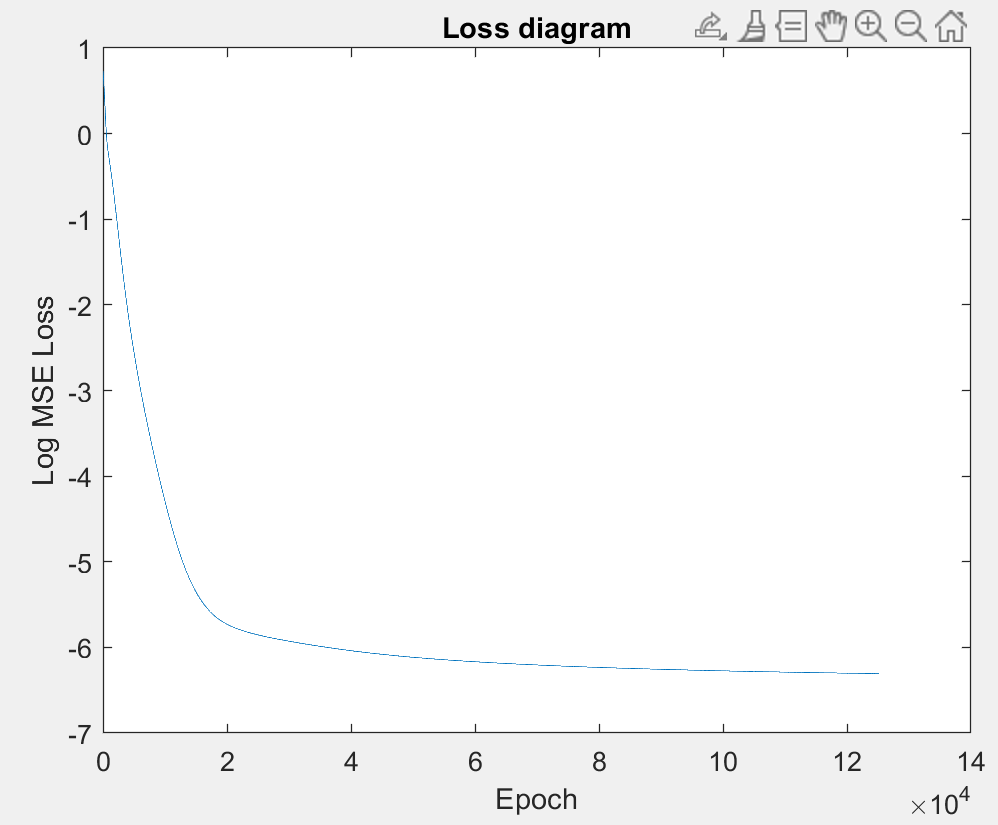
\includegraphics[width=0.4\textwidth]{smallLR_1.PNG}\label{fig:f1}}
  \hfill
  \subfloat[Large $\alpha$]{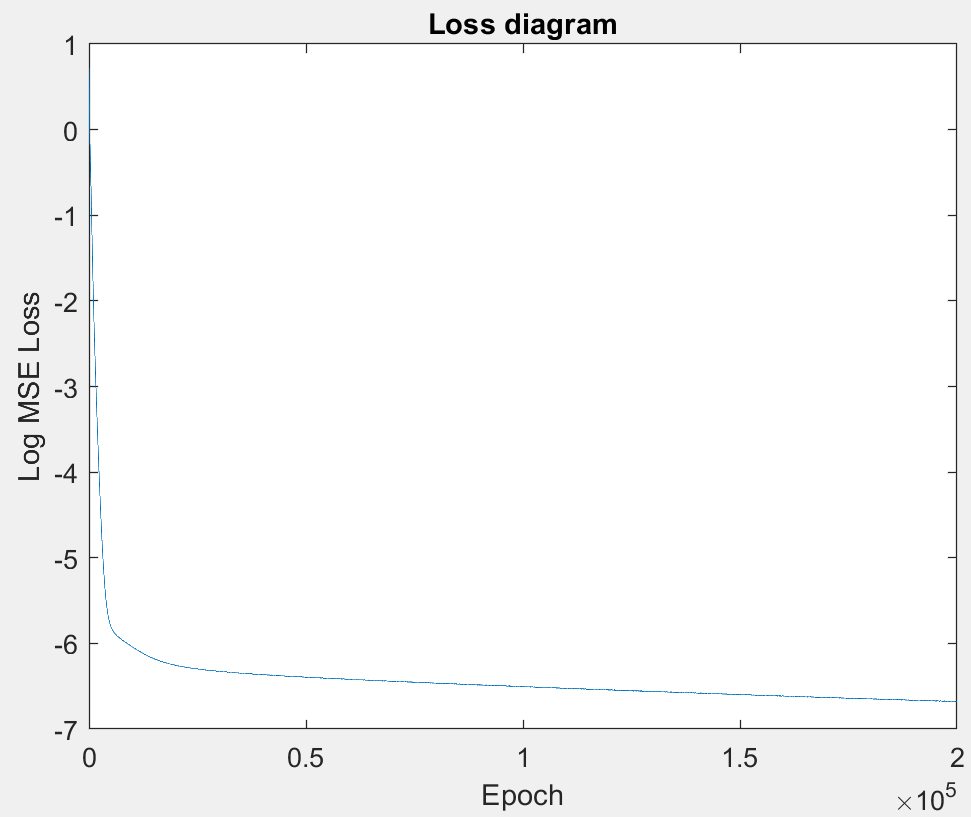
\includegraphics[width=0.4\textwidth]{largeLR_1.PNG}\label{fig:f2}}
  \caption{Loss vs. Epoch plots demonstrating the effect of learning rate}
\end{figure}

The batch sizes were 200 or 20,000. The latter value is the size of the entire dataset and thus corresponds to performing regular gradient descent. 200 is a somewhat typical value for a batch size with stochastic gradient descent, but this can likely be optimized.\\
The activation function of the first layer was also varied between a sigmoid function and ReLu. The latter performed better as a rule.\\

The other hyperparameters were fixed for these tests. \\
The maximum number of epochs (iterations of the training loop) was $2 \times 10^4$. This is smaller than typical, which resulted in larger loss values as the network is often not fully converged to its optimal solution; for this reason a must larger maximum could be justified, but would dramatically increase the time required to conduct this testing.\\
The epsilon used was $5 \times 10^{-6}$. This breaks out of the training loop if the norm of two adjacent $\overrightarrow{\theta}$s is below this value.\\
The dataset size was initially 2,000, but was bumped up to the recommended 20,000 for this testing campaign. $20\% $ of this dataset was set aside for testing while the rest was used for training.\\

\section{Results}
In this section, let's call the network that is built into Matlab `network 1' and our custom model `network 2'. These will allow us to label and discuss these results more easily. Let's begin with the results of the testing campaign for network 2. Again, the hyperparameters not listed in the chart were fixed at $max_{epoch} = 20,000$, $\epsilon = 0.000005$, and $N = 20,000$.

\begin{center}
\begin{tabular}{||c c c c c c c||} 
 \hline
 Test & $\Psi_0$ & $J$ & $\alpha$ & $M$ & run time & final loss \\ [0.5ex] 
 \hline\hline
 1 & ReLu &  30 & $2*10^{-3}$ & 200 & 105.0 & 0.002295\\ 
 \hline
 2 & ReLu & 30 & $2*10^{-3}$ & 20,000 & 524.7 & 0.002308\\
 \hline
 3 & ReLu & 30 & $5*10^{-4}$ & 200 & 107.1 & 0.005991\\
 \hline
 4 & ReLu & 30 & $5*10^{-4}$ & 20,000 & 528.9 & 0.005510\\
 \hline
 5 & ReLu & 3 & $2*10^{-3}$ & 200 & 22.1 & 0.002833\\
 \hline
 6 & ReLu & 3 & $2*10^{-3}$ & 20,000 & 59.0 & 0.002553\\
 \hline 
 7 & ReLu & 3 & $5*10^{-4}$ & 200 & 22.4 & 0.014274\\
 \hline
 8 & ReLu & 3 & $5*10^{-4}$ & 20,000 & 64.9 & 0.017604\\
 \hline
 9 & Sigmoid &  30 & $2*10^{-3}$ & 200 & 138.8 & 0.009123\\ 
 \hline
 10 & Sigmoid & 30 & $2*10^{-3}$ & 20,000 & 576.7 & 0.008796\\
 \hline
 11 & Sigmoid & 30 & $5*10^{-4}$ & 200 & 136.5 & 0.023443\\
 \hline
 12 & Sigmoid & 30 & $5*10^{-4}$ & 20,000 & 573.9 & 0.036606\\
 \hline
 13 & Sigmoid & 3 & $2*10^{-3}$ & 200 & 29.2 & 0.012064\\
 \hline
 14 & Sigmoid & 3 & $2*10^{-3}$ & 20,000 & 73.0 & 0.012938\\
 \hline 
 15 & Sigmoid & 3 & $5*10^{-4}$ & 200 & 28.7 & 0.432972\\
 \hline
 16 & Sigmoid & 3 & $5*10^{-4}$ & 20,000 & 70.1 & 0.410554\\[1ex] 
 \hline
\end{tabular}
\end{center}

First we notice that the use of stochastic gradient descent (where $M=200$) cuts the run time by a factor of 3 to 5 and on average does not change the network's performance. However, the error diagrams show a more involved story. The diagrams in figure 2 show the difference between the two: the smoother profile occurs under full gradient descent because the derivatives are updated based on the entire dataset's average. The rougher occurs when we use stochastic gradient descent because we pick a batch and only those influence the direction of our derivatives; this may cause rapidly changing directions.\\

\begin{figure} [!tbp]
  \centering
  \subfloat[With Stochastic Gradient Descent]{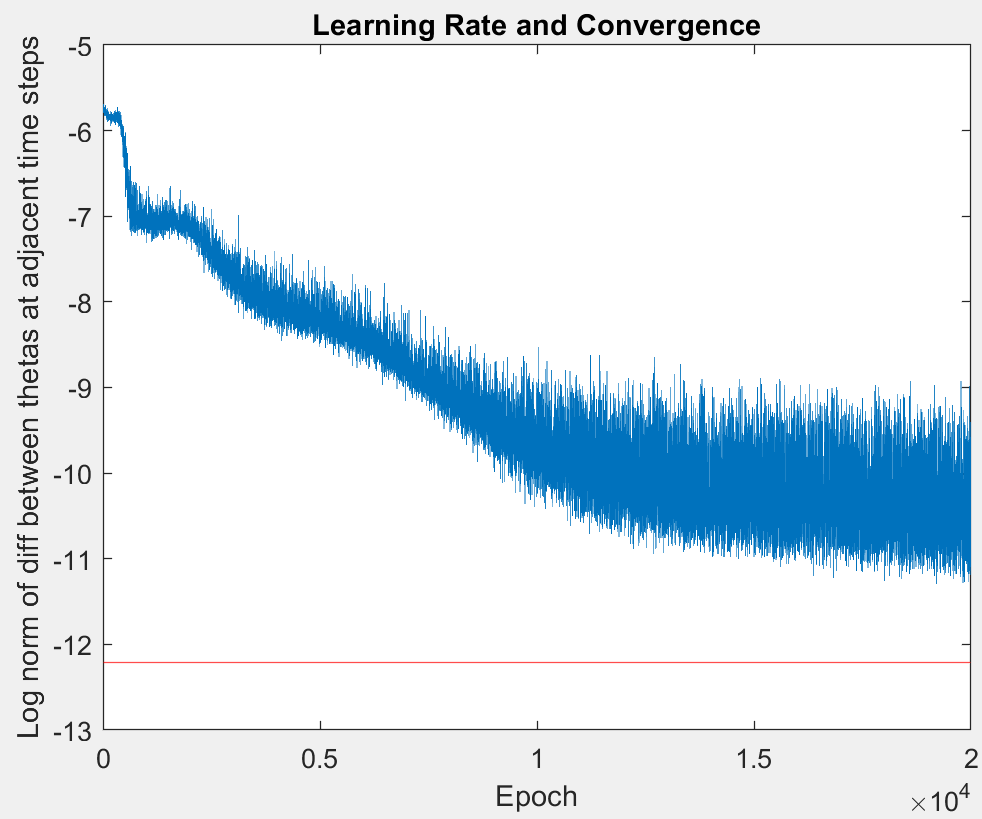
\includegraphics[width=0.4\textwidth]{sgd.PNG}\label{fig:f5}}
  \hfill
  \subfloat[Without Stochastic Gradient Descent]{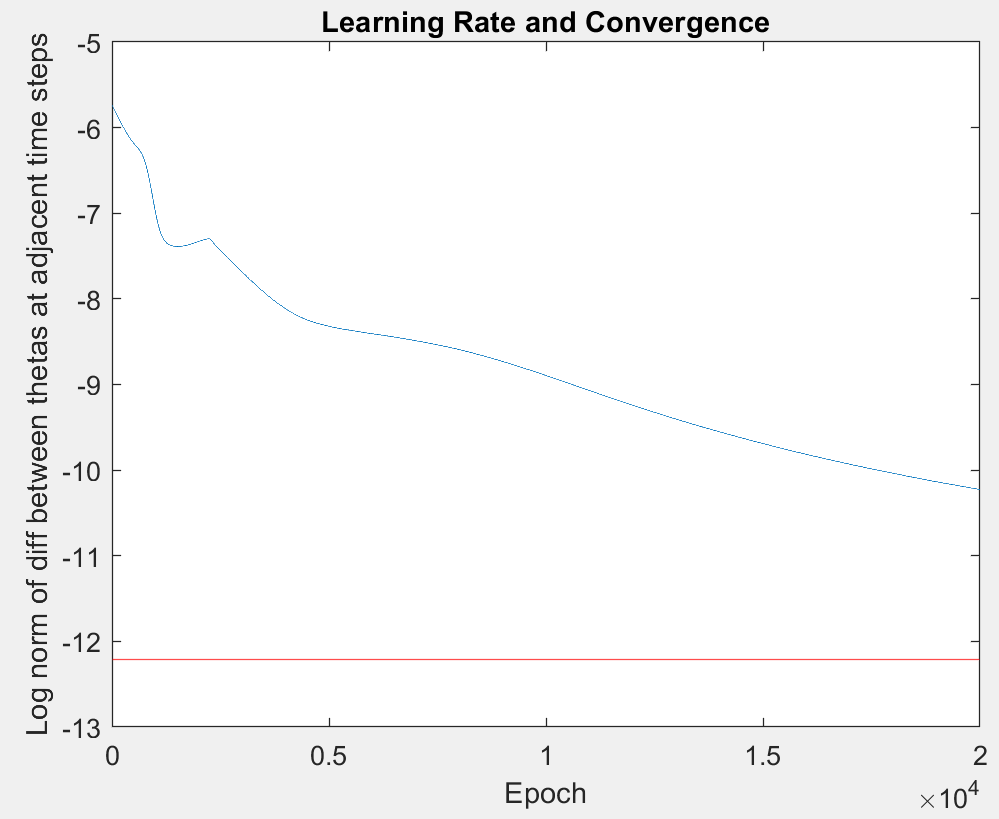
\includegraphics[width=0.4\textwidth]{gd_full.PNG}\label{fig:f6}}
  \caption{Convergence of $\overrightarrow{\theta}$ Plots}
\end{figure}

Next we notice that the sigmoid activation function is outperformed in both metrics by ReLu in every tested case. The error plots generated by such tests supports the conclusion that sigmoid does not approximate the Black Scholes function as well; its errors are skewed left and the plots themselves show that the price prediction trend has a negative concavity where the concavity should be zero. See figure 3 for a demonstration.\\ 

\begin{figure} [!tbp]
  \centering
  \subfloat[Error Distribution]{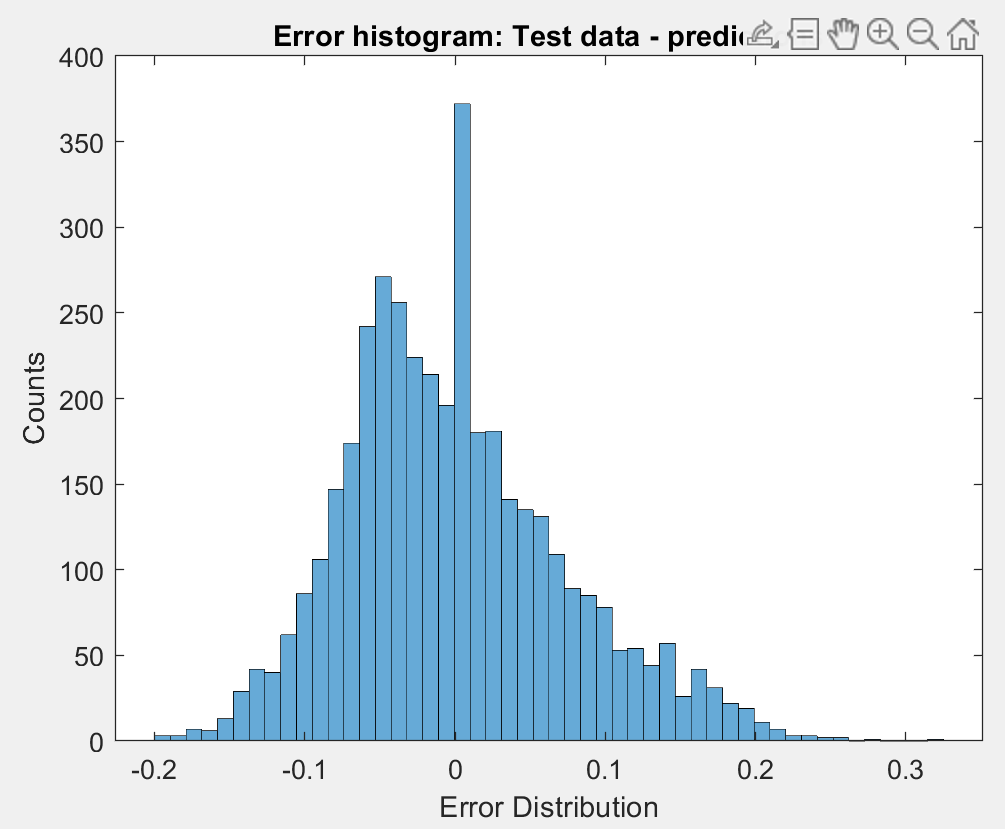
\includegraphics[width=0.4\textwidth]{sigmoid_error.PNG}\label{fig:f3}}
  \hfill
  \subfloat[Price Predictions vs. Price]{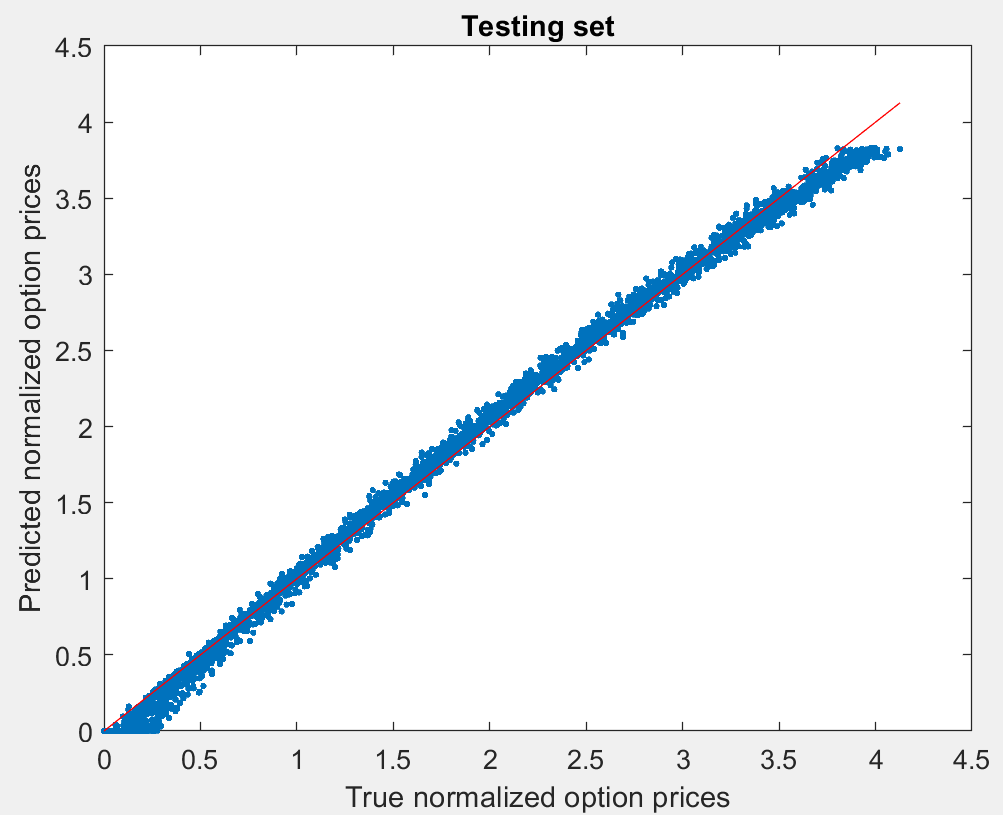
\includegraphics[width=0.4\textwidth]{sigmoid_pred_plot.PNG}\label{fig:f4}}
  \caption{Sigmoid activation's poor performance}
\end{figure}

Thirdly, we notice that decreasing the number of neurons in the ReLu case did not make a large difference in the quality of the results but greatly reduced the computation required. \\

Not shown in the chart is which terminal condition was exercised by each run: every test performed above ended its training by reaching the maximum number of epochs and not by their $\theta$'s reaching the convergence limit. This means that if $max_{epoch}$ were increased, we would likely see more uniform loss results with more variable run times, but this would have given the tests with the smaller learning rate a better shot at converging and even outperforming their larger learning rate counterparts. For example, test 8 was repeated with a larger $max_{epoch}$; it converged after 55,000 epochs, 158.9 seconds, and achieved a final loss of 0.003321--a result that is comparable to tests 3 and 4 with the larger learning rate. For this reason, the campaign conducted herein may be misleading regarding the effect of the learning rate.\\

Now let's include some results from network 1 for the sake of comparison and elaboration from section 2. Many of the hyperparameters listed for network 2 either do not apply to network 1 or are much more complicated and implemented in a different way. For example, instead of setting a single value for $\alpha$, there is an initial learning rate set to $8.8 \times 10^{-3}$ and several variables about how it should decrease in a piece wise manner every 4 steps in such a manner to satisfy several additional constraints. The ones that are the same, however, are the dataset and its size, and the batch size for Stochastic gradient descent is still 200.\\

\begin{center}
\begin{tabular}{||c c c c c c||} 
 \hline
 Test & Activation & Layers & Neurons & run time & final loss \\ [0.5ex] 
 \hline\hline
 1 & ReLu & 1 & 3 & 22.6 & 0.000676\\ 
 \hline
 2 & ReLu & 1 & 30  & 23.2 & 0.000761\\
 \hline
 3 & ReLu & 1 & 100 & 24.3 & 0.000996\\
 \hline
 4 & ReLu & 6 & 3  & 33.9 & 0.000669\\
 \hline
 5 & ReLu & 6 & 30  & 44.0 & 0.000311\\
 \hline
 6 & ReLu & 6 & 100 & 53.2 & 0.000247\\
 \hline 
 7 & Sigmoid & 1 & 3  & 26.4 & 0.002290\\ 
 \hline
 8 & Sigmoid & 1 & 30 & 26.6 & 0.000703\\
 \hline
 9 & Sigmoid & 1 & 100  & 29.2 & 0.000948\\
 \hline
 10 & Sigmoid & 6 & 3  & 48.7 & 1.531545\\
 \hline
 11 & Sigmoid & 6 & 30  & 57.5 & 0.004917\\
 \hline
 12 & Sigmoid & 6 & 100  & 68.6 & 0.000792\\
 \hline 
\end{tabular}
\end{center}

The first thing we noticed is that test 10 utterly failed to converge. The next is how much smaller both the run times and losses are compared to network 2! Network 1 is doing things network 2 cannot (2 is fixed at one layer) while also doing it quickly and well. The next thing we notice is that the relationship between the number of layers and the number of neurons is not linear--when the number of layers increases, whether the loss increases or decreases depends also on the number of neurons. There is likely some complicated topology here and finding the optimal value for even one hyperparameter would take a good bit of tinkering; such an optimal value is likely a function of the other hyperparameters.\\

\section{Concluding Remarks}
Which neural network is better? The answer is obvious: the network that uses Matlab's built in functions and objects has been optimized in almost every conceivable way, and it outperforms our first attempt at a network handily in every metric. It is one to twelve times faster, achieves five to ten times lower losses, and is more general, modular, and capable. By `general', I mean that the custom network relies on hand-calculated derivatives for the loss function, and as such, changing which activation function one uses, let alone adding more hidden layers, becomes time consuming at best and infeasible in even moderately large cases.\\

A positive for network 2 is that it could be used to illustrate more basic principles of neural networks. One basic feature that could be added without much more work would be some scheme to dynamically adjust the learning rate, $\alpha$. Such technical schemes exist in various research literature, but largely remained outside the scope of this project. Should the author's clinic project pertain to neural networks and similar topics, such schemes, along with many other potential improvements, will also be considered. For example, could $\alpha$ be implemented in such a way as to be dynamic for each parameter? Such schemes may exist in computer science literature, but likely remain unexplored as applied to finance.\\

Thank you for reading/listening. This concludes the author's final project of Advanced Topics in Financial Mathematics taught by Dr. Ruihua Liu in the fall of 2022. Below is the code that implemented the above-described networks.\\

\section{Code}
\subsection{Data set generator script} As with the Matlab neural network, this program was changed only marginally from a web-based publication that used the same principles to price barrier options.
\begin{lstlisting}
%Cj Destefani
%Data set generating script for project 3 option pricing NN
%Pick parameter ranges and find the 'exact' value with the BSM equation.

% Option parameter ranges.
% The first value defines the lower bound and the second value is the upper bound.
moneyness = [0.5 5]; % S0/K
maturity = [0.1 2]; % time in years
rate = [0.01 0.10]; %interest rate between 1% and 10%
sigma = [0.05 0.5]; %volatility
dividend = [0 0.03]; %dividend rate between 0% and 3%
Datasetsize=20000;

%generate quasi-random numbers for parameter spacing
Quasi = sobolset(5,'Skip',1024);
Quasi = scramble(Quasi,'MatousekAffineOwen');
inputs = Quasi(1:Datasetsize,:); % Initial samples

%scale each random number to be in the proper ranges
inputs(:,1) = inputs(:,1)*(moneyness(2)-moneyness(1))+moneyness(1);   % Moneyness S0/K
inputs(:,2) = inputs(:,2)*(maturity(2)-maturity(1))+maturity(1);      % Maturity time
inputs(:,3) = inputs(:,3)*(rate(2)-rate(1))+rate(1);                  % Interest rate
inputs(:,4) = inputs(:,4)*(sigma(2)-sigma(1))+sigma(1);               % Volatility 
inputs(:,5) = inputs(:,5)*(dividend(2)-dividend(1))+dividend(1);      % Dividend rate
 
% Use the Black_Scholes_Merton formula to calculate the call option prices.
Price =zeros(length(inputs),1);
for i = 1:size(inputs,1)
    Price(i) = blsprice(inputs(i,1),1,inputs(i,3),inputs(i,2),inputs(i,4),inputs(i,5));
end

save('Training02.mat', 'Price', 'inputs');  
\end{lstlisting}

\subsection{Network 1} The second line below gives a link to a more involved project that used a very similar code.\\

\begin{lstlisting}
%modified code from the Barrier option pricing with the Heston Model page:
% https://www.mathworks.com/help/fininst/deep-learning-to-approximate-barrier-option-pricing.html
% cj destefani 11/19

% Load the training data.
load('Training02.mat', 'Price', 'inputs');  
%Define the neural network
numFeatures = size(inputs,2); %should give 5
w=100; %width of network
layers = [
    featureInputLayer(numFeatures,Normalization='zscore')    
    fullyConnectedLayer(w,WeightsInitializer='he') %initialized as normal RVs with mean 0 and var 2/sample size
    %sigmoidLayer
    reluLayer
    %{
    fullyConnectedLayer(w,WeightsInitializer='he')
    %sigmoidLayer
    reluLayer
    fullyConnectedLayer(w,WeightsInitializer='he')
    %sigmoidLayer
    reluLayer
    fullyConnectedLayer(w,WeightsInitializer='he')
    %sigmoidLayer
    reluLayer
    fullyConnectedLayer(w,WeightsInitializer='he')
    %sigmoidLayer
    reluLayer
    fullyConnectedLayer(w,WeightsInitializer='he') %final hidden layer
    %sigmoidLayer
    reluLayer
    %}
    fullyConnectedLayer(1,WeightsInitializer='he') %output/regression layer
    reluLayer
    regressionLayer];

n = size(Price,1);
c = cvpartition(n,Holdout=1/5);     % Hold out 1/5 of the data set for testing
XTrain = inputs(training(c),:);     % 4/5 of the input for training
YTrain = Price(training(c),:);      % 4/5 of the target for training
XTest = inputs(test(c),:);          % 1/5 of the input for testing
YTest = Price(test(c),:);           % 1/5 of the target for testing

nTrain = size(XTrain,1); %size of training set
idx = randperm(nTrain,floor(nTrain*0.1)); % 10% validation data
XValidation = XTrain(idx,:);
XTrain(idx,:) = [];
YValidation = YTrain(idx,:);
YTrain(idx,:) = [];

opts = trainingOptions('adam', ...
    MaxEpochs=30, ...
    Shuffle='every-epoch', ...
    Plots='none', ...
    Verbose=false, ...
    VerboseFrequency=50, ...
    MiniBatchSize=200, ... %batch size. was 265
    ValidationData={XValidation,YValidation}, ...
    ValidationFrequency=50, ...
    ValidationPatience=Inf, ...
    L2Regularization=1.9e-7, ...
    InitialLearnRate=8.8e-3, ...
    LearnRateSchedule='piecewise', ...
    LearnRateDropPeriod=4, ...
    LearnRateDropFactor=0.128, ...
    SquaredGradientDecayFactor=0.55, ...
    GradientDecayFactor=0.62);
    
% Train the network.
net = trainNetwork(XTrain,YTrain,layers,opts);

% Test the network.
YPred = predict(net,XTest);

% Measure the results and plot the outputs.
fprintf('The MSE is: %2.6f\n', mean((YTest - YPred).^2))

figure
histogram(YTest - YPred, 50)
xlabel('Error Distribution')
ylabel('Counts')

figure
plot(YTest,YPred,'.',[min(YTest),max(YTest)],[min(YTest),max(YTest)],'r')
xlabel('Scaled Actual Price')
ylabel('Scaled Predicted Price')
title('Predictions on Test Data')
\end{lstlisting}

\subsection{Custom NN} Note that there is a Boolean variable for whether or not to use stochastic gradient descent or not. Using it improves performance by a factor of 3 even on small datasets, and the benefits will be greater on larger datasets.\\

\begin{lstlisting}
%project 3_02
%try to make everything from scratch
%NN option pricing project
%Cj Destefani, project and presentation due 12-5-22.
% Dr. Liu's Topics in Financial Mathematics, UD Financial Math.

%% Basic set up
SGD=true; %if true, uses stochastic GD, otherwise uses full GD.
useRelu=true; %boolean. if true, use relu, if false use sigmoid for first activation function.
smallSetSize=false; %which dataset to use

if smallSetSize
    load('Training01.mat', 'Price', 'inputs');  %2,000 option prices and inputs
else
    load('Training02.mat', 'Price', 'inputs'); %20,000 option prices and inputs
end

%Set hyperparameters
J=3; %width of the network
alpha=5*10^-4; %learning rate
M=200; %batch size
epoch_max=2*10^4; %training automatically stops after this many iterations
epsilon=5*10^-6; %training also stops if two sets of parameters are this close to each other

%activation functions
sig= @(x) 1./(1+exp(-x)); %sigmoid activation function
%dsig= @(x) sig(x).*(1-sig(x)); %derivative of sigmoid
relu= @(x) max(0,x); %rectified linear unit activation function
drelu= @(x) (x>0)*1; %derivative of relu, is activation function: 1 if x>0, 0 otherwise.

% split data into training and testing
N=size(inputs,1); %total dataset size
L=zeros(epoch_max,1); %saves loss function at each epoch
ntheta=zeros(epoch_max,1); %saves norms of the difference between parameters at step l and l+1. 
epoch=0; %store epoch number
X=inputs; %rename so these can be played with without damaging original dataset
Y=Price;
Ntrain=floor(N*.8); %number of datapoints in training set ~80% of data to train, and 20% to test.
Ntest=N-Ntrain;
idx0=randperm(N,Ntrain); %pick out indexes of training data points
x_Tr=X(idx0,:); %use those idices to get input and output data
y_Tr=Y(idx0);
X(idx0,:)=0; %clear the ones set aside for training
Y(idx0)=0;
idx1=find(Y); %finds the index of the nonzero elements
x_Te=X(idx1,:); %put the rest in testing sets
y_Te=Y(idx1);
s=sqrt(Ntest)/2; %stretch or squish distribution of starting weights and biases

%% Run NN
%set initial weights
W0=randn(J,5)/s; %randomly initialize weights. W0 connects inputs and hidden layer
W1=randn(1,J)/s; %W1 is weights connecting hidden layer and output
b0=randn(J,1)/s; % biases for hidden layer
b1=randn(1,1)/s+1; % bias for output
dLdw1=zeros(J,1);
dLdb0=zeros(J,1);
dLdw0=zeros(J,5);

while true
epoch=epoch+1; %increment counter

% Feed forward through network
u=W0*x_Tr' + b0; %first function
if useRelu
    v=relu(u); %first activation
else
    v=sig(u); %alternative first activation function: performs worse
end
w=W1*v+b1; %final layer
y_hat=relu(w); %final activation

%calculate loss
prod0=y_Tr'-y_hat; %this is not actually a product, but it is used in multiple places and will take less memory if given a name
L(epoch) = mean(prod0.^2); %loss function is MSE, saved at each iteration

% calculate derivatives in order to perform either gradient descent or stochastic gradient descent
if SGD
    %incorporate batch size so that we use stochastic gradient descent:
    idx2=randperm(Ntrain,M); %pick out indexes of training data points
    v_short=v(:,idx2); %will be a MxJ matrix
    x_Tr_short=x_Tr(idx2,:);
    w_short=w(idx2);
    u_short=u(:,idx2);

    %back propagation with SGD--approximate derivatives
    prod1=2*(prod0(idx2)).*drelu(w_short);
    dLdb1=mean(prod1); %same for both useRelu and ~useRelu since final activation is Relu in both cases
    for j=1:J
        dLdw1(j)=mean(prod1.*v_short(j,:)); %also same in both activation cases
        if useRelu
            prod2=prod1.*W1(j).*drelu(u_short(j,:)); %store these here to reduce total number of multiplications network performs
            dLdb0(j)=mean(prod2);
            for k=1:5
                dLdw0(j,k)=mean(prod2.*x_Tr_short(:,k)'); %depends on both j and k so is inside a loop for each
            end
        else
            prod2=prod1.*W1(j).*v_short(j,:).*(1-v_short(j,:)); % dsig(u_short(j,:)); this alternative notation is equivalent to dsig, but is faster
            dLdb0(j)=mean(prod2);
            for k=1:5
                dLdw0(j,k)=mean(prod2.*x_Tr_short(:,k)');
            end
        end
    end
else
    %back propagation--gradient descent--uses 'exact' derivates. does not shorten any vectors, but otherwise operates the same as above.
    prod1=2*(prod0).*drelu(w);
    dLdb1=mean(prod1);
    for j=1:J
        dLdw1(j)=mean(prod1.*v(j,:));
        if useRelu
            prod2=prod1.*W1(j).*drelu(u(j,:));
            dLdb0(j)=mean(prod2);
            for k=1:5
                dLdw0(j,k)=mean(prod2.*x_Tr(:,k)');
            end
        else
            prod2=prod1.*W1(j).*v(j,:).*(1-v(j,:)); %dsig(u(j,:));
            dLdb0(j)=mean(prod2); 
            for k=1:5
                dLdw0(j,k)=mean(prod2.*x_Tr(:,k)');
            end
        end
    end
end

% iterate parameters with either gradient descent or Stochastic gradient descent
theta=[W0(:); b0; W1'; b1]; % 7J+1 parameters long
gradL=-1*[dLdw0(:); dLdb0; dLdw1; dLdb1];
theta2 = theta- alpha*gradL; 

%repackage parameters and use in next iteration
b1 = theta2(7*J+1); %last entry
W1 = theta2(6*J+1:7*J)'; % J entries before that
b0 = theta2(5*J+1:6*J); % J entries before that
W0 = reshape(theta2(1:5*J),[J,5]); %first 5J entries

%terminal conditions
ntheta(epoch)=norm(theta2-theta);
if ntheta(epoch)<epsilon
    L(epoch+1:epoch_max)=[]; %remove extra empty entries if it ends early
    ntheta(epoch+1:epoch_max)=[]; 
    fprintf("Solution converged in %d iterations.\n",epoch)
    break;
end
if epoch>=epoch_max
    fprintf("Solution did not converge after %d iterations.\n", epoch)
    break;
end
end

%% evaluate test data set and plot results
if useRelu
    y_fin=relu(W1*relu(W0*x_Te' + b0) + b1); %create predicted y values with test data
else
    y_fin=relu(W1*sig(W0*x_Te' + b0) + b1); %create predicted y values with test data
end
mseTest = mean((y_Te' - y_fin).^2);
fprintf("Final error: %2.6f\n",L(epoch))
fprintf("MSE on test data: %2.6f\n",mseTest)

%{
figure
plot(y_Tr,y_hat,'.')
xlabel("True normalized option prices");
ylabel("Predicted normalized option prices");
title('Training set')
%}

figure
histogram(y_Te' - y_fin, 50)
xlabel('Error Distribution')
ylabel('Counts')
title('Error histogram: Test data - predictions')

figure
plot(y_Te,y_fin,'.',[min(y_Te),max(y_Te)],[min(y_Te),max(y_Te)],'r')
xlabel("True normalized option prices");
ylabel("Predicted normalized option prices");
title('Testing set')

figure
plot(log(1:epoch),log(L))
xlabel("Log Epoch");
ylabel("Log MSE Loss");
title('Loss diagram')

figure
plot(1:epoch,log(ntheta))
hold on
yline(log(epsilon),'r')
xlabel("Epoch");
ylabel("Log norm of diff between thetas at adjacent time steps");
title('Learning Rate and Convergence')
\end{lstlisting}

\end{document}